\section{Problem Description}
Imagine the following scenario: A multinational tech company YanSoftware with offices worldwide wants to incentivise employees to cycle and visit the gym more often. It introduces these goals to contribute to the environment and improve general employee health. Several implementation options are available, such as posters, emails, websites, employee workshops, and campaigns; but another common method the business can adopt is that of a loyalty scheme. YanSoftware may have one or many of such schemes within their business to manage. Loyalty methods available to them range from the basic stamp/sticker book, to the more modern smartcards (Fig. 1).

Commonly, simple paper-based systems are adopted by businesses due to low cost and implementation times; nonetheless systems like these have several issues. Some individuals may lose their stamp booklets, some are concerned about the environmental impact associated with printing many cards of paper; furthermore, it is important to note that paper-based solutions are not very secure and open to abuse.

An opportunity exists for a general-purpose system to encompass loyalty programs via use of up-and-coming Near-Field Communication (NFC) technologies that are integrated inside modern smart phones. Moreover, elements of gamification can be added as an extra dimension of loyalty to corporate persuasive technologies. (e.g. unlocking better rewards as they level-up, essentially playing versus themselves)

\begin{figure}[h!]
    \centering
    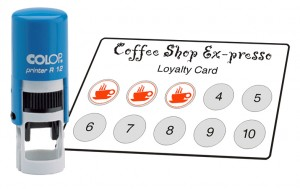
\includegraphics[width=0.5\textwidth]{img/Loyalty-card.jpg}
    \qquad
    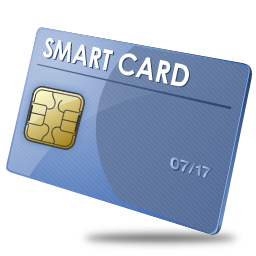
\includegraphics[width=0.3\textwidth]{img/smartcard.png}
    \caption{A paper stamp card \& smart card}%
\end{figure}
\clearpage{}

\clearpage{}

\subsection{Rationale}
The smartphone is now a staple item which many people cannot leave their home without. As of 2014, there is a worldwide user-base of approximately 1.75 billion smartphone devices~\cite{smartUsers}. Migration to phones allow the business to have a central hub of all of their loyalty schemes, eradicating the need for paper. This means that issues relating to paper-based systems, such as printing paper (environmental impact) and people losing their stampcards are no longer an issue. Moreover, businesses will now have the option to track use and monitor their schemes for further analysis. This grants them insight into how many users they have, allowing them to adjust loyalty schemes appropriately.

On the other hand the proposed solution is not without some problems of its own. For instance, not everybody owns a smartphone, so hybrid smartphone/paper solutions will need to be considered. Additionally, there exists specific disadvantages of smartphones, such as dependence on battery life and an internet connection.


\subsection{Aim}
The aim of this project is to develop a general purpose solution using a smartphone that supports businesses in creating, managing and deploying a simple loyalty scheme - using gamification elements to engage the users. The specific technology chosen is NFC in phones running the Android operating system. 


\subsection{Objectives}
\begin{itemize}
    \item Research the state-of-art surrounding NFC technology within loyalty and gamification systems
    \item Examine and Analyse the current smartphone solutions available to manage loyalty systems
    \item Design and implement the solution
    \item Perform an evaluation on the different interaction cases and interfaces
    \item Look into the future possibilities of the system and the infrastructural requirements to support them
\end{itemize}


\subsection{Similar Developments}
There exist some similar mobile-based solutions to the one proposed, such as Apple's \emph{PassBook}. Passbook is an iOS exclusive application that allows users to save their generic cards (i.e. boarding passes, event tickets, loyalty cards etc.) Though also a general purpose solution, there is a distinction on the technologies used (QR/Barcode Scanning) and the interactions presented to the users - For example, Passbook entails the one-way interaction of simply scanning barcodes. By adopting the two-way possibilities provided by NFC, richer interactions can be built and allow inter-communication between devices.

Other loyalty applications also exist, some using some combination of NFC or gamification elements; nonetheless they are specific to their associated brand. Starbucks' application on iOS is one such example (Fig. 2), offering users a digital QR version of their Starbucks card (Fig. 2c) and a medium to collect rewards in the form of stars. These stars, along with the account balance can be used to claim rewards and beverages. The opportunity of our proposed solution is to make an encompassing general-purpose solution that any business, big or small, can use to simply implement a loyalty program.


\begin{figure}[h!]
  \centering
    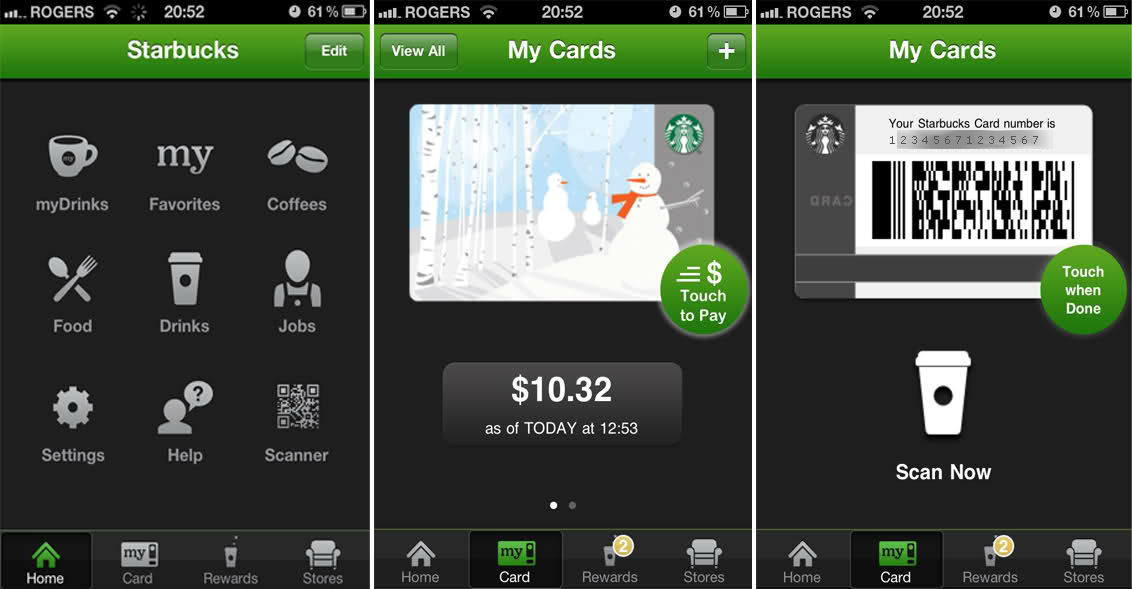
\includegraphics[width=1\textwidth]{img/starbucks-image-2.jpeg}
      \caption{Starbucks application for iOS (a) The menu of the Starbucks app(b) The card and available balance (c) The bar-code presented to the baristas to scan}
\end{figure}

\section{Resources}
\subsection{Technologies}
\subsubsection{Android Platform}
Android is a smartphone operating system developed by Google. Along with Windows Mobile OS and Apple's iOS, these three operating systems are the biggest players in the global smartphone market. Android was chosen because most devices are equipped with an NFC chip and have well supported APIs regarding Host Card Emulation (See 4.1.4 Host Card Emulation). With the introduction of iOS8 and the iPhone 6, Apple now has support for NFC payments; however the APIs are unavailable to developers at this time and as a result, cannot be used. Windows Phone has similar NFC libraries to Android, but was not chosen due to it's low market share (2.5\% as a pose to Android's 84.7\%)\cite{marketShare}. 
\subsubsection{Android SDK}
The Android Software Development Kit (SDK) Will be required to develop, implement and test the Android applications. There are several methods that can be chosen regarding Android application development without having to use Google's JAVA SDK. Unfortunately, due to the specific dependencies on Google's NFC APIs, development will need to be done using the JAVA SDK.
\subsubsection{Google+ API (Sign in with Google)}
This API allows users to use the system by means of their Google account. The rationale is to allow people to \emph{one-click sign in} without having to worry about registering and logging into a new account. It is more secure having the user's account details on Google's servers, rather than creating and storing information for a brand new account. On the other hand, If users deem appropriate in the post-implementation evaluation, a separate registration process will be considered.
\subsubsection{Host Card Emulation (HCE)}
NFC chips can be placed into Card Emulation mode in such a way (ISO 14443) that a reader classifies it in the same manner as a smartcard.\cite{ecosystem}. Implementation of the system is dependent on use of this NFC facet. \emph{Android Kitkat} supports this mode within its APIs.
\subsection{Android Devices}
For most cases of Android development, the bundled emulator with Google's Android SDK is sufficient; however due to the project's dependence on the NFC chip, at least two physical (preferably differently branded) devices need to be used. One will be running the Loyalty Manager, whilst others will be running the Loyalty Reader. Both devices must at least have the \emph{Kitkat 4.4} iteration of Android in order to use Host Card Emulation.
\subsection{Users}
A group of individuals will be required to assess the different interfaces and interaction use-cases. Smooth interactions are important in order to both encourage and optimise use in fast-serving environments (i.e a coffee shop). General members of the public would be used for the Loyalty Reader, whereas input from business owners would be most valuable on the Loyalty Manager. 
